\documentclass[11pt]{article}
	\usepackage[T1]{fontenc}
    % Nicer default font (+ math font) than Computer Modern for most use cases
    % \usepackage{mathpazo}

    % Basic figure setup, for now with no caption control since it's done
    % automatically by Pandoc (which extracts ![](path) syntax from Markdown).
    \usepackage{graphics}
    % We will generate all images so they have a width \maxwidth. This means
    % that they will get their normal width if they fit onto the page, but
    % are scaled down if they would overflow the margins.
    \makeatletter
    \def\maxwidth{\ifdim\Gin@nat@width>\linewidth\linewidth
    \else\Gin@nat@width\fi}
    \makeatother
    \let\Oldincludegraphics\includegraphics
    % Set max figure width to be 80% of text width, for now hardcoded.
    \renewcommand{\includegraphics}[1]{\Oldincludegraphics[width=.8\maxwidth]{#1}}
    % Ensure that by default, figures have no caption (until we provide a
    % proper Figure object with a Caption API and a way to capture that
    % in the conversion process - todo).
    \usepackage[center,bf]{caption}
    % \DeclareCaptionLabelFormat{nolabel}{}
    % \captionsetup{labelformat=nolabel}

    \usepackage{adjustbox} % Used to constrain images to a maximum size 
    \usepackage{xcolor} % Allow colors to be defined
    \usepackage{enumerate} % Needed for markdown enumerations to work
    \usepackage{geometry} % Used to adjust the document margins
    \usepackage{amsmath} % Equations
    \usepackage{amssymb} % Equations
    \usepackage{textcomp} % defines textquotesingle
    % Hack from http://tex.stackexchange.com/a/47451/13684:
    \AtBeginDocument{%
        \def\PYZsq{\textquotesingle}% Upright quotes in Pygmentized code
    }
    \usepackage{upquote} % Upright quotes for verbatim code
    \usepackage{eurosym} % defines \euro
    \usepackage[mathletters]{ucs} % Extended unicode (utf-8) support
    \usepackage[utf8x]{inputenc} % Allow utf-8 characters in the tex document
    \usepackage{fancyvrb} % verbatim replacement that allows latex
    \usepackage{grffile} % extends the file name processing of package graphics 
                         % to support a larger range 
    % The hyperref package gives us a pdf with properly built
    % internal navigation ('pdf bookmarks' for the table of contents,
    % internal cross-reference links, web links for URLs, etc.)
    \usepackage{hyperref}
    \usepackage{longtable} % longtable support required by pandoc >1.10
    \usepackage{booktabs}  % table support for pandoc > 1.12.2
    \usepackage[inline]{enumitem} % IRkernel/repr support (it uses the enumerate* environment)
    \usepackage[normalem]{ulem} % ulem is needed to support strikethroughs (\sout)
                                % normalem makes italics be italics, not underlines
   	\usepackage[]{authblk}
   	\usepackage{cite}
    \usepackage{graphicx}
    \usepackage{hyperref}
    \usepackage{amsmath}
    \usepackage{amsthm}
    \usepackage{amssymb}
    \usepackage{bm}
    \usepackage{bbm}
    \usepackage{algorithmicx}
    \usepackage{algorithm}
    \usepackage{algpseudocode}
    \usepackage{array}
    \usepackage{booktabs}
    \usepackage{multirow}
    \usepackage{makecell}
    \usepackage{color}
    \usepackage{tabularx,ragged2e,booktabs,caption}

   	\makeatletter
    \def\@maketitle{%
    \newpage
      \null
      \vskip 2em%
      \begin{center}%
      \let \footnote \thanks
        {\Large\bfseries \@title \par}%
        \vskip 1.5em%
        {\normalsize
          \lineskip .5em%
          \begin{tabular}[t]{c}%
            \@author
          \end{tabular}\par}%
        \vskip 1em%
        {\normalsize \@date}%
      \end{center}%
      \par
      \vskip 1.5em}
    \makeatother


\newtheorem{theorem}{Theorem}






\title{EE 232E Project 2\\Social Network Mining}
\author{Hengjie~Yang, Sheng~Chang, Wendi~Cui, and Tianyi~Liu
}


\date{\today}


\begin{document}
\maketitle

\section{A brief tutorial on how to use this template}
\Large\textcolor{red}{\bf{Please remove the tutorial section in the final manuscript\\ by commenting, i.e. $\%(something)$}}


\subsection{Figures}
Figure insertion is shown in Fig \ref{example_fig}.
\begin{figure}[h]
\centering
\scalebox{0.7}{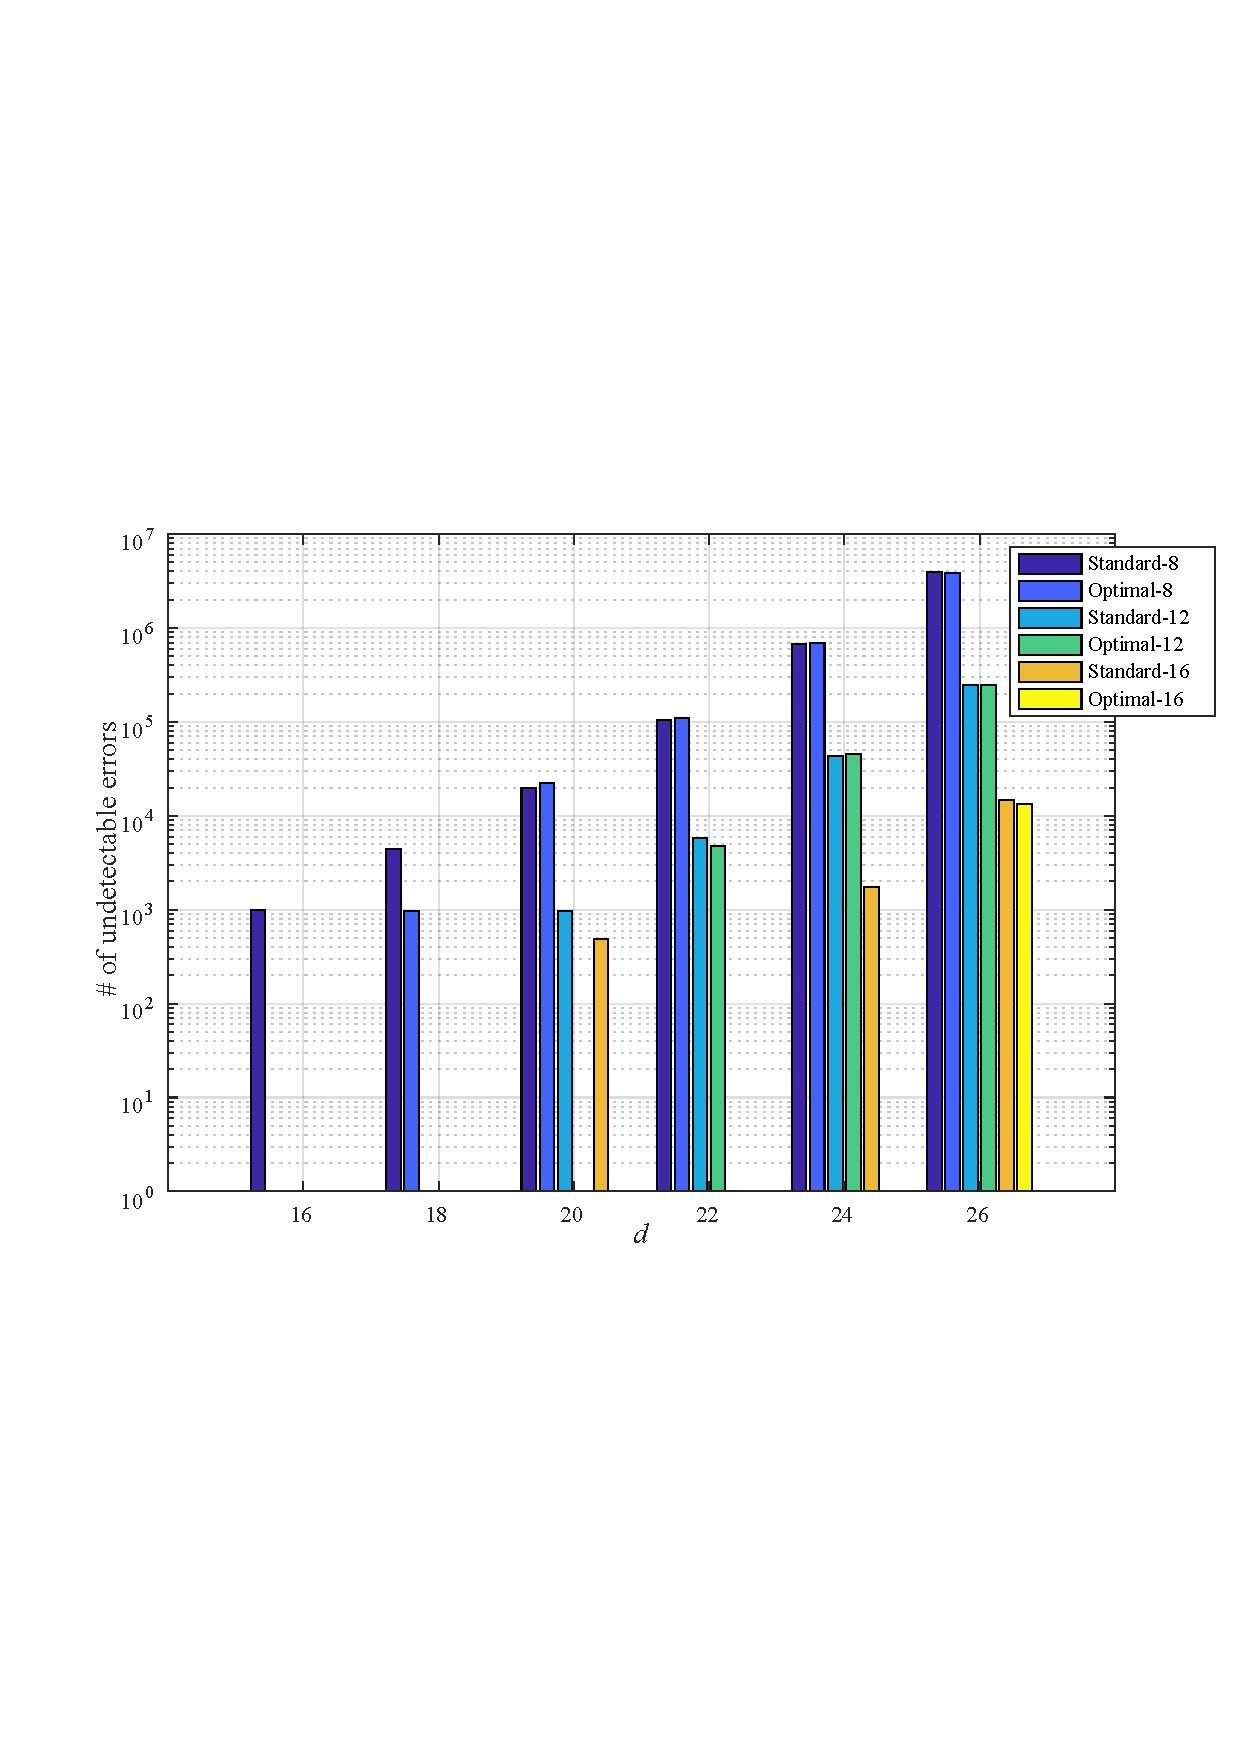
\includegraphics{Figures/spectrum_bar.pdf}}
\caption{An example of figure insertion}
\label{example_fig}
\end{figure}

\subsection{Equations}
An example of equations is given as follows.
\begin{theorem}
Let $a$, $b$, $c$ denote the sides of a triangle, respectively. If $a\perp b$, the pythagoras theorem is given as follows.
\begin{align}
c^2 = a^2 + b^2
\end{align}
\end{theorem}

\subsection{Tables}
An example of tables is shown in Table \ref{example_table}.
\renewcommand\arraystretch{1.1}
\begin{table}[h]
\center
\caption{Standard CRC Codes versus Optimal CRC Codes for Convolutional Code $G=(561~753)$ with $n=504$ Bits}
\scalebox{0.9}{
\begin{tabular}{r|c|c|cccccc}
\hline
\multirow{2}{*}{Name} & \multirow{2}{*}{Gen. Poly.} & \multicolumn{7}{c}{Undetected Error Distance Spectrum} \\
\cline{3-9}
 & & $d$ & 16 & 18 & 20 & 22 & 24 & 26 \\\hline\hline
Standard-8 & \multicolumn{1}{l}{0x19B} & & 983 & 4387 & 19909 & 105000 & 672724 & 3972970\\
Optimal-8 & \multicolumn{1}{l}{0x19D} & & 0 & 979 & 22349 & 111304 & 686314 & 3830340\\\hline
Standard-12 & \multicolumn{1}{l}{0x180F} & & 0 & 0 & 969 & 5815 & 42893 & 245211 \\
Optimal-12 & \multicolumn{1}{l}{0x108B} & & 0 & 0 & 0 & 4793 & 45795 & 246729\\\hline
Standard-16 & \multicolumn{1}{l}{0x11021} & & 0 & 0 & 484 & 0 & 1765 & 14752\\
Optimal-16 & \multicolumn{1}{l}{0x1F8FD} & & 0 & 0 & 0 & 0 & 0 & 13240\\\hline
\end{tabular}}
\label{example_table}
\end{table}


\section{Facebook network}


\subsection{Structural properties of the facebook network}


\subsection{Personalized network}


\subsection{Core node’s personalized network}

\subsubsection{Community structure of core node’s personalized network}

\subsubsection{Community structure with the core node removed}

\subsubsection{Characteristic of nodes in the personalized network}


\subsection{Friend recommendation in personalized networks}

\subsubsection{Neighborhood based measure}


\subsubsection{Friend recommendation using neighborhood based measures}

\subsubsection{Creating the list of users}

\subsubsection{Average accuracy of friend recommendation algorithm}





\section{Google+ Network}

\subsection{Community structure of personal networks}




\end{document}







